\chapter{Moving Obstacle Avoidance}
In this chapter we present an Obstacle Avoidance alghorithm based on Adaptive Model Predictive Control. First we introduced the case-study model, then we designed the controller and the method of decision-making. Finally we verified the proposed strategy in different scenarios.

\section{Problem Formulation}
The collision avoidance problem is very dependent on the vehicle modeling since it is a requirement for  adaptive MPC law design. Figure \ref{fig:obstacleAvoidance} illustrates a typical scenario of overtaking of a moving obstacle. The maneuver from the driver is to temporarily move to another lane, drive past the obstacle, and move back to the original lane afterward. 
% COLLISION AVOIDANCE FIGURE
\begin{figure}[!h]
	\centering
	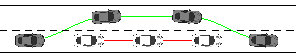
\includegraphics[width=\textwidth]{./figure/obstacleAvoidance/obstacleAvoidance.pdf}
	\caption{Problem description of collision avoidance on a road with only two lanes.}
	\label{fig:obstacleAvoidance}
\end{figure}

This is possible if and only if there is a free lane or  sufficient space for overtaking the obstacle. In the case the road is busy with vehicles, the ATLASCAR2 must slow down and adapts its speed to that of the closest obstacle until the scenario changes.

\subsection{Car-like Model}
The model used in this part of the thesis should take into account the kinematic and dynamic aspects of the vehicle. Here, we present a non linear mathematical model of a vehicle used for the development of a collision avoidance system. The model has four states and two inputs:
\begin{equation}
\begin{array}{cc}
\vec{x}=\begin{bmatrix}
x\\y\\\theta\\v 
\end{bmatrix},\qquad 
\vec{u}=\begin{bmatrix}
T\\\delta 
\end{bmatrix}
\end{array} 
\end{equation}

where $(x,y)$ are the global coordinates of the contact point between the rear wheel and the ground, $\theta$ is the heading angle of the car body with respect to the $x$-axis and $v$ is the linear speed of the car (positive). The manipulated variables are $T$ the throttle (positive when accelerating/negative when braking) and $\delta$ the steering angle of the front wheel with respect to the vehicle ($0$ when aligned with car, counterclockwise positive). Figure \ref{fig:car_model} illustrates the applied nonlinear bicycle model and the related parameters.
% BICYCLE MODEL
\begin{figure}[!h]
	\centering
	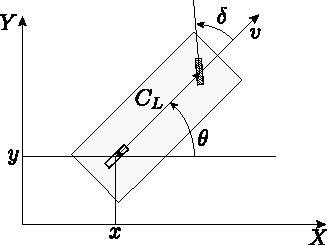
\includegraphics[width=0.65\textwidth]{./figure/car_model.pdf}
	\caption{Bicycle model of a car (adapted from \cite{siciliano}).}
	\label{fig:car_model}
\end{figure}

The ATLASCAR2 can be modeled using the non-linear kinematic bicycle model described by the following equations of motion \cite{safety} \cite{swarms}:
\begin{equation}
\label{eqn:dynamics_model_obstacle_avoidance}
\left \{ \begin{array}{llll}
\dot{x} = v\cos(\theta)\\
\dot{y} = v\sin(\theta)\\
\dot{\theta} =\dfrac{v}{C_L}\tan(\delta)\\
\dot{v} =0.5 \cdot T
\end{array} 
\right .
\Longrightarrow 
\begin{array}{llll}
\dot{\vec{x}} = \vec{f}(\vec{x},\vec{u})\\
\vec{y} = \vec{g}(\vec{x},\vec{u})
\end{array}
\end{equation}

where $C_L$ is the car length. When the velocity is zero then the rate of change of heading angle is zero, that is, it is not possible to change the vehicle's orientation
when it is not moving. If the front wheel is orthogonal to the back wheel, i.e. the steering angle is $\frac{\pi}{2}$, the ATLASCAR2 cannot move forward and the model enters an undefined region. In order to simplify the model, it is assumed that only the front wheel can be steered. Moreover, in this chapter it is assumed that the ATLASCAR2 does not slip, so any slippage is thus considered as an external disturbance. Under this assumption, the slip angle is zero, meaning that the velocity is directed along the heading of the vehicle. In particular the rate of change of heading angle is referred to as turn rate which can be evaluated with a gyroscope. This yaw rate can also be deduced from the angular velocity of the wheels on the left- and right-hand sides of the vehicle which therefore rotate at different speeds because follow arcs of different radius. We can write the non-holonomic constraint which is an expression for velocity in the vehicle's $y$-direction in the world coordinate frame as follows:
\begin{equation}
	\dot{y}\cos\theta-\dot{x}\cos\theta=0.
\end{equation}

This equation cannot be integrated to form a
relationship between $x,y$ and $\theta$. In order to use an MPC controller, the state space model needs to be linearized with a first order approximation and also re-written in a more compact form:
\begin{equation}
\label{eqn:dynamics_model_non_linear}
\begin{array}{llll}
\dot{\vec{x}} = \vec{f}(\vec{x},\vec{u})\\
\vec{y} = \vec{g}(\vec{x},\vec{u})
\end{array} \Longrightarrow
\begin{array}{ll}
\dot{\vec{x}} =\vec{A}_c \vec{x}+ \vec{B}_c \vec{u}\\
\vec{y} =\vec{C}_c \vec{x} + \vec{D}_c \vec{u}
\end{array}
\end{equation}
where the matrices $\vec{A}_c$, $\vec{B}_c$, $\vec{C}_c$ and $\vec{D}_c$ are obtained as follows:
\begin{equation}
\begin{array}{ccc}
\vec{A}_c=\displaystyle\frac{\partial \vec{f}(\vec{x},\vec{u})}{\partial \vec{x}}=\begin{bmatrix}
0&0&-v\sin(\theta)&\cos(\theta)\\
0&0&v\cos(\theta)&\sin(\theta)\\
0&0&0&\tan(\delta)/C_L\\
0&0&0&0
\end{bmatrix},
\\\\
\vec{B}_c=\displaystyle\frac{\partial \vec{f}(\vec{x},\vec{u})}{\partial \vec{u}}=\begin{bmatrix}
0&0\\
0&0\\
0&\dfrac{v}{C_L}\big(\tan(\delta)^2+1\big)\\
0.5&0
\end{bmatrix},
\\\\
\vec{C}_c=\displaystyle\frac{\partial \vec{g}(\vec{x},\vec{u})}{\partial \vec{u}} = \mathbf{I}_4, 
\qquad
\vec{D}_c=\frac{\partial \vec{g}(\vec{x},\vec{u})}{\partial \vec{u}}=\mathbf{0}_{4\times2}.
\end{array}
\end{equation} 
The simple linearized approximation of the system to describe the dynamics of the ATLASCAR2 will be evaluated at the operating conditions. Note also that the system we are considering is a linear state-space model whose dynamics vary as a function of certain time-varying parameters. The system to be controlled is usually modeled by a discrete state-space model in the MPC literature. Therefore, (\ref{eqn:dynamics_model_non_linear})
is transformed into a discrete state-space model to be used by the Model Predictive Controller:
\begin{equation}
\label{eqn:dynamics_ss_obstacle_avoidance_dis}
\begin{array}{ll}
\dot{\vec{x}} =\vec{A}_c \vec{x}+ \vec{B}_c \vec{u}\\
\vec{y} =\vec{C}_c \vec{x} + \vec{D}_c \vec{u}
\end{array}
\Longrightarrow
\begin{array}{rr}
{\vec{x}}(k+1) =\vec{A}_d \vec{x}(k)+ \vec{B}_d \vec{u}(k)\\
\vec{y}(k) =\vec{C}_d \vec{x}(k) + \vec{D}_d \vec{u}(k)
\end{array}
\end{equation}

where $\vec{A}_d$ and $\vec{B}_d$ are the state and control matrices for the discrete state-space equation, respectively, which can be calculated with the Euler method as
\begin{equation}
\vec{A}_d = e^{\vec{A}_cT_s},\qquad \vec{B}_d = \int_{kT_s}^{(k+1)T_s} e^{\vec{A}_c[(k+1)T_s-\eta]}\vec{B}_c d\eta
\end{equation}

where $T_s$ is the sampling interval for the discrete state-space model. The matrices $\vec{C}_d$ and $\vec{D}_d$ are equivalent to those in the continuous case. For simplicity, we assume that all the states are measurable and the ATLASCAR2 drives east with a constant speed at the nominal operating point. 

In the scenario that we are going to consider, the road is straight and our vehicle stays in the middle of the center lane when not passing. Without losing generality, the ATLASCAR2 passes an obstacle both to the right and to the left lane depending on where it is placed on the road. We create also a safe zone around the obstacles so that the vehicle does not get too close to the obstacle when passing it.

\section{Design of Adaptive Model Predictive Control}
We designed a Model Predictive Controller that can make the ATLASCAR2 maintain a desired velocity and stay in the middle of center lane. We used an Adaptive MPC controller because it handles the nonlinear vehicle dynamics more effectively than a traditional MPC controller; in fact, the latter uses a constant plant model but the former allows us to provide a new plant model at each control interval. Because the new model describes the plant dynamics more accurately at the new operating condition, an adaptive MPC controller performs better than a traditional MPC controller. 

In practice, at each control interval, the adaptive MPC controller updates the plant model and the nominal conditions. Once updated, the model and the conditions remain constant over the prediction horizon. In motion planning that uses adaptive MPC, it is common to formulate the constrained control problem as a real-time optimization problem subject to hard constraints on plant variables and soft constraints on outputs; at the beginning, we specified the constraints for the manipulated variables: to prevent the ATLASCAR2 from accelerating or decelerating too quickly, we added an hard constraint on the throttle rate of change and another one on the steering angle rate of change. We used an approach that takes advantage of the ability of MPC to handle constraint explicitly. Figure \ref{fig:flowchart} shows a conditional state machine designed for higher-level behavior planning.
% FLOWCHART
\begin{figure}[!t]
	\centering
	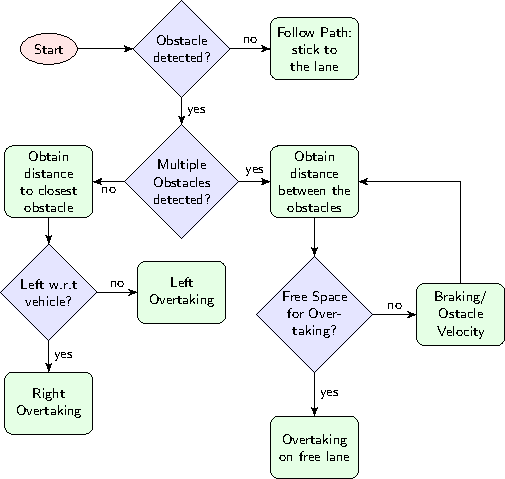
\includegraphics[width=0.90\textwidth]{./figure/flowchart/flowchart.pdf}
	\caption{Behaviour planning conditional flowchart.}
	\label{fig:flowchart}
\end{figure}

When an obstacle is detected, it defines an area on the road (in terms of constraints) that the ATLASCAR2 must not enter during the prediction horizon. At the next control interval the area is redefined based on the new positions of the vehicle and the obstacle until passing is completed.

To define the area to avoid, we used the following mixed Input/Output constraints:
\begin{equation}
\label{eqn:mixed_IO_constraints}
\vec{E}\vec{u}+\vec{F}\vec{y}\leq \vec{G}
\end{equation}
where $\vec{u}$ and $\vec{y}$ are respectively the manipulated variable vector and the output variable vector, while $\vec{E},\vec{F},\vec{G}$ are the constraint matrices that can be updated when the controller is running. 

Five constraints were defined:
\begin{enumerate}
	\item upper bound on the $y$-coordinate (left boundary of the road);
	\item lower bound on the $y$-coordinate (right boundary of the road);
	\item constraint for obstacle avoidance; although no obstacle is considered in the nominal condition, we must add this virtual constraint here because we cannot change the dimensions of the constraint matrices at run time;
	\item upper bound on the $x$-coordinate (position of the closest obstacle);
	\item lower bound on the $x$-coordinate (position of the ATLASCAR2).
\end{enumerate}
The matrices for the above inequality are the following:
\begin{equation}
\vec{E}= 
\begin{bmatrix}
0&0\\
0&0\\
0&0\\
0&0\\
0&0
\end{bmatrix},
\qquad
\vec{F}=\begin{bmatrix}
0&1&0&0\\
0&-1&0&0\\
cS&-1&0&0\\
1&0&0&0\\
-1&0&0&0\\
\end{bmatrix},
\qquad
\vec{G}=
\begin{bmatrix}
W/2\\W/2\\-cI\\x_{\max}\\x_{\min}
\end{bmatrix}
\end{equation}

where $W$ is the width of the road, $cI$ and $cS$ are the required parameters such that the ATLASCAR2 must be above the line formed from the vehicle to safe zone corner for left/right passing and finally $x_{\max}$ represents the position of the closest obstacle in the case there is not free space for the overtaking (otherwise $x_{\max}=+\infty$) while $x_{\min}$ depicts the location of our vehicle. Figure \ref{fig:constraint} illustrates the constraints that are computed at each $T_s$ in the case of a left overtaking.
% FIGURE CONSTRAINT
\begin{figure}[!h]
	\centering
	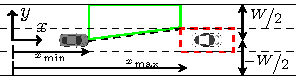
\includegraphics[width=\textwidth]{./figure/constraint/constraint.pdf}
	\caption{Constraints in the case of left overtaking.}
	\label{fig:constraint}
\end{figure}

\section{Simulation Results}
The performances of the proposed adaptive MPC based vehicle control method are demonstrated in four simulation examples. We tried to choose parameters that were as close as possible to a real situation: the sampling time used in the discretization of the system is $T_s=\SI{0.02}{s}$ while the values of the prediction and the control horizon are respectively $p_H=25$ and $c_H=5$. 

In all simulations, the distance between the front and rear axles is $C_L=\SI{5}{m}$ and the width of the vehicle is $C_W=\SI{2}{m}$. The saturation ranges of the control inputs are: the steering angle rate of change lies in $\big[-\frac{\pi}{30}, +\frac{\pi}{30}\big]$ rad/s while in order to prevent the ATLASCAR2 from accelerating or decelerating too quickly, we impose an hard constraint of \SI{2.5}{m/s^2} on the throttle rate of change.

Moreover we are using a constant reference signal for the velocity of $v=\SI{20}{m/s}$ ($\approx\SI{72}{km/h}$).
Note that the blue paths in Figures \ref{fig:obstacleAvoidance_one_obstacle}, \ref{fig:obstacleAvoidance_random}, 	\ref{fig:obstacleAvoidance_six_obstacles}, \ref{fig:obstacleAvoidance_no_overtaking} and \ref{fig:braking} are known only at the end of the simulations but we have decided to report the entire trajectory that the vehicle will perform in every frame. The overall framework for a multiple moving obstacle avoidance is depicted in the Figure \ref{fig:MovingObstacleAvoidance}.
% OVERALL SCHEME ONE MOVING OBSTACLE
\begin{figure}[!h]
	\centering
	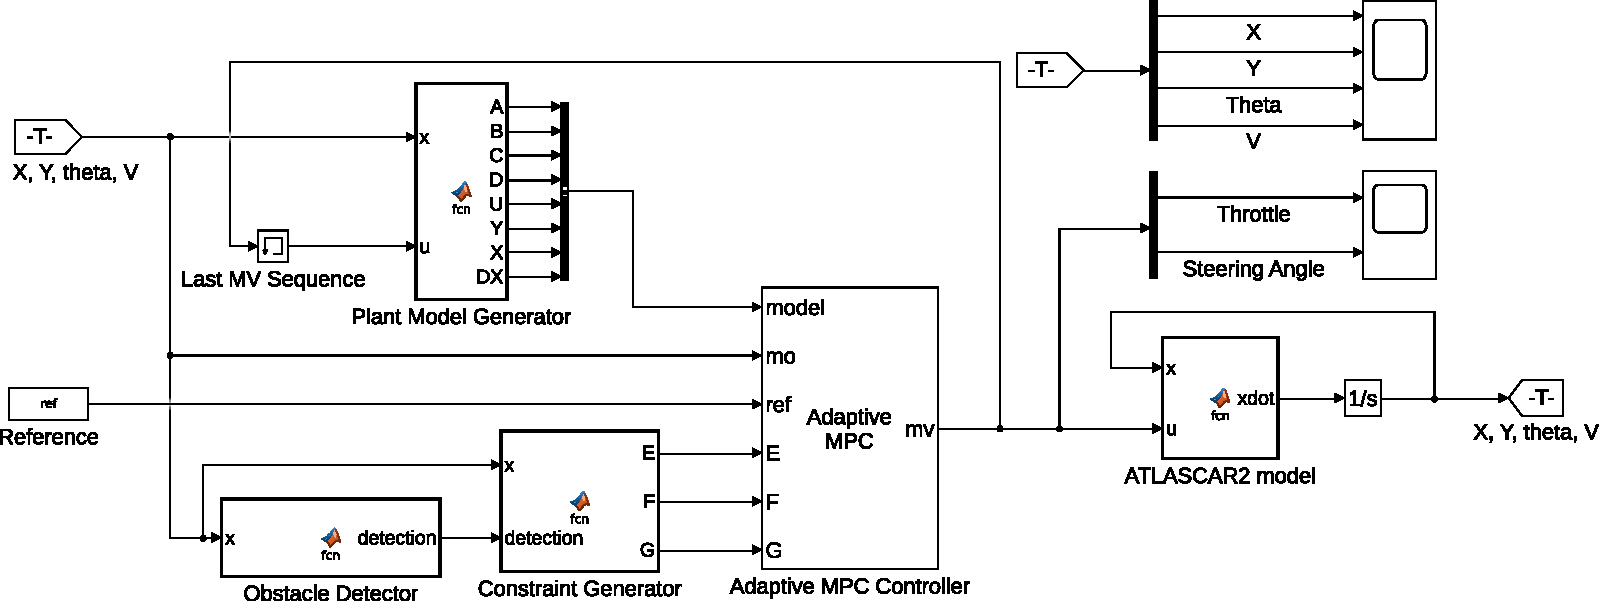
\includegraphics[width=\textwidth]{./figure/MovingObstacleAvoidance.pdf}
	\caption{Overall procedure scheme moving obstacle avoidance.}
	\label{fig:MovingObstacleAvoidance}
\end{figure}

All the simulations are done in MATLAB and Simulink. MATLAB is used for loop-shaping. Simulink is used as a testing environment.  Moreover, the MATLAB Model Predictive Toolbox is used. The controller will be tested in the same Simulink environment as the classical controller. Note that all these blocks have been implemented through the S-functions (types of dynamically linked subroutines for Simulink).

\subsection{One Moving Obstacle - Right Overtaking}
In this first simulation
(Figure \ref{fig:obstacleAvoidance_one_obstacle}) the ATLASCAR2 drives in the middle of the center lane while the road is completely free and when there is an obstacle, the vehicle passes it only using the right lane (the same simulation can be launched so that the car goes over to the left fast lane). In this example the obstacle has a constant speed of \SI{8}{m/s} and moves in the same direction as the ATLASCAR2. We assume that the LIDAR sensor can detect an obstacle \SI{30}{m} in front of the vehicle.
The red dashed block around the obstacle represents a safe zone used to evaluate the restrictions so that, even if there is a small margin of error in the manuever, there is always a safe distance between the ATLASCAR2 and the nearby vehicle.
% ONE MOVING OBSTACLE
\begin{figure}[h!]
	\centering
	\begin{minipage}[t]{\textwidth}
		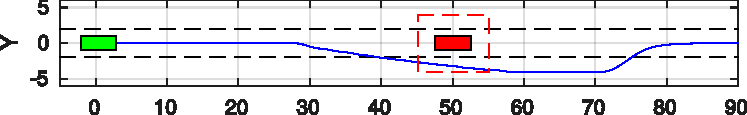
\includegraphics[width=\textwidth]{./figure/one_obstacle_right_overtaking/overtaking_start.pdf}
	\end{minipage}
	\begin{minipage}[t]{\textwidth}
		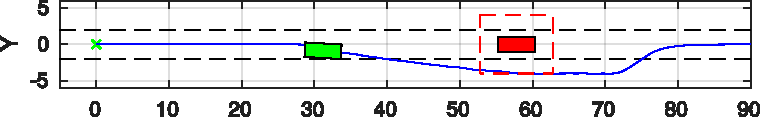
\includegraphics[width=\textwidth]{./figure/one_obstacle_right_overtaking/overtaking_middle.pdf}
	\end{minipage}
	\begin{minipage}[t]{\textwidth}
		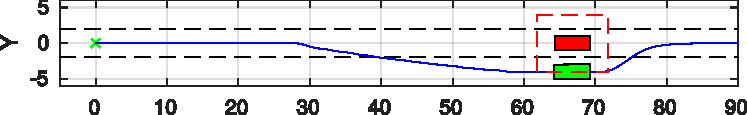
\includegraphics[width=\textwidth]{./figure/one_obstacle_right_overtaking/overtaking_middle_end.pdf}
	\end{minipage}
	\begin{minipage}[t]{\textwidth}
		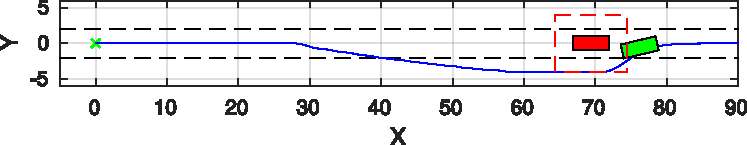
\includegraphics[width=\textwidth]{./figure/one_obstacle_right_overtaking/overtaking_end.pdf}
	\end{minipage}
	\caption{Simulation of right overtaking with one moving obstacle that moves in the same direction as the vehicle.}
	\label{fig:obstacleAvoidance_one_obstacle}
\end{figure}

Algorithm \ref{alg:rightOvertaking} summarizes the main steps to compute custom constraints for the obstacle; when the vehicle detects the obstacle, the constraints are computed.

In other words the constraints are evaluated as follows:
\begin{itemize}
	\item if the ATLASCAR2 is already in the adjacent lane, it uses the safety zone as the constraint (line \ref{line:safety_zone});
	\item otherwise the vehicle must be above the line formed from the ATLASCAR2 to safe zone corner for right passing (lines \ref{line:corner1} and \ref{line:corner2});
	\item if the vehicle is parallel to the obstacle (line \ref{line:safety_zone_parallel}), it  uses the safety zone as the constraint;
	\item finally if it has passed the obstacle, it uses the inactive constraint to go back to the center lane (line \ref{line:inactive}).
\end{itemize}

% ALGORITHM FOR RIGHT OVERTAKING OF ONE MOVING OBSTACLE
\begin{algorithm}[!h]
	\caption{Right Overtaking if an obstacle is detected}
	\small
	\begin{algorithmic}[1]
		\Function{RightOvertaking}{car, obstacle, road}
		\State $x_\text{min} \gets \text{car}X $,  $x_\text{max} \gets +\infty$;
		\State obsYrr = Obstacle.RearRightSafeY;
		\State obsXrr = Obstacle.RearRightSafeX;
		\If{ATLASCAR2 is behind the obstacle} 
		\If{ATLASCAR2 is in the adjacent lane}
		\State $cS \gets 0$; $cI \gets \text{obsYrr}$; \label{line:safety_zone}
		\Else
		\State $cS \gets \text{tan}(\text{atan2}(\frac{\text{obsYrr}-\text{ carY}}{\text{obsXrr}-\text{carX}},1))$; \label{line:corner1}
		\State $cI \gets \text{obsYrr}-cS*\text{obsXrr}$;\label{line:corner2}
		\EndIf
		\Else
		\If{ATLASCAR2 is parallel to the obstacle}
		\State $cS \gets 0$; $cI \gets \text{obsYrr}$;\label{line:safety_zone_parallel}
		\Else
		\State $cS \gets 0$; $cI \gets W/2$;\label{line:inactive}
		\EndIf
		\EndIf
		\State \Return $x_\text{min}$, $x_\text{max}$, $cI$, $cS$
		\State \text{Update matrices $\vec{E},\vec{F}$ and $\vec{G}$}
		\EndFunction
	\end{algorithmic}
	\label{alg:rightOvertaking}
\end{algorithm}

In this simulation only the first three constraints are necessary because there is enough space for the overtaking without braking (the fourth and fifth constraints don't change). The first two constraints are constant and represent the left and right boundary of the road (upper and lower bound on the $y$-coordinate). The third constraint is useful to define a region where the vehicle can navigate; it consists of two parameters ($cS$ and $cI$) that are calculated in the algorithm depending on where the vehicle is located with respect to the obstacle. After calculating these parameters, the matrices $\vec{E}$, $\vec{F}$ and $\vec{G}$ are updated so that the MPC can process the new optimal input. 

Finally we can analyze time signals of the ATLASCAR2 in the simulation of right overtaking of one moving obstacle. Figures \ref{fig:longitudinal_one_moving} and \ref{fig:lateral_one_moving} illustrate the longitudinal and lateral position of the vehicle with respect to time, showing a constant trend with respect to the $x$ component, while a shift from 0 can be noted regarding the $y$ coordinate due to the overcoming of the obstacle. 
To confirm a uniform trend, the speed of the ATLASCAR2 remains fairly constant. Obviously it is possible to note from Figure \ref{fig:velocity_one_moving} that the velocity decreases very little during the first part of the overtaking phase, and then come back to the cruising speed in the second part. Instead from the remaining Figures \ref{fig:throttle_one_moving}, \ref{fig:delta_one_moving} and \ref{fig:theta_one_moving} we can observe that the throttle $T$ and the steering angle $\delta$ respect the limits we imposed while the heading angle $\theta$ is used to describe the direction the ATLASCAR2 is pointing.
% RESULTS ONE MOVING OBSTACLE
\begin{figure}[!t] %vs changes to t instead of b
	\begin{minipage}[t]{0.5\textwidth}
		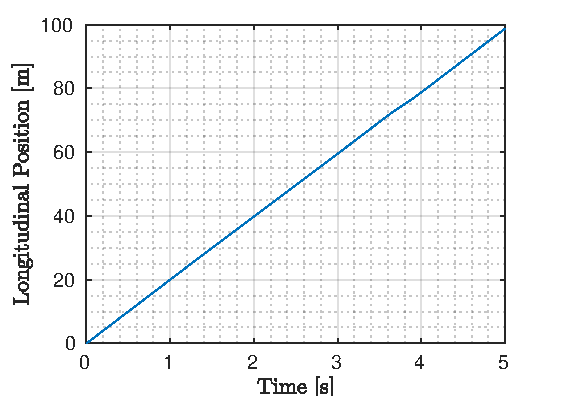
\includegraphics[width=\textwidth]{../../MATLAB/one_obstacle_right_overtaking/figure/LongitudinalPositionVsTime.pdf}
		\subcaption{}\label{fig:longitudinal_one_moving}
	\end{minipage}
	\begin{minipage}[t]{0.5\textwidth}
		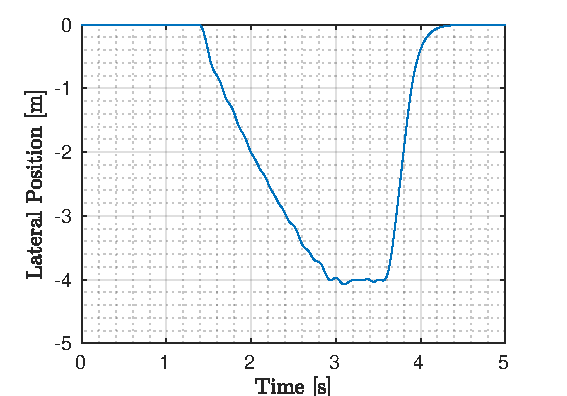
\includegraphics[width=\textwidth]{../../MATLAB/one_obstacle_right_overtaking/figure/LateralPositionVsTime.pdf}
		\subcaption{}\label{fig:lateral_one_moving}
	\end{minipage}
	\begin{minipage}[t]{0.5\textwidth}
		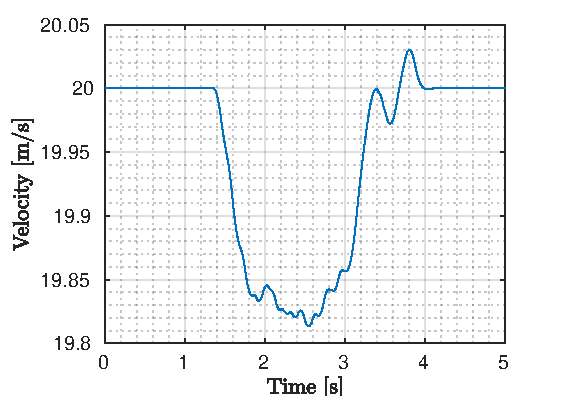
\includegraphics[width=\textwidth]{../../MATLAB/one_obstacle_right_overtaking/figure/VelocityVsTime.pdf}
		\subcaption{}\label{fig:velocity_one_moving}
	\end{minipage}
	\begin{minipage}[t]{0.5\textwidth}
		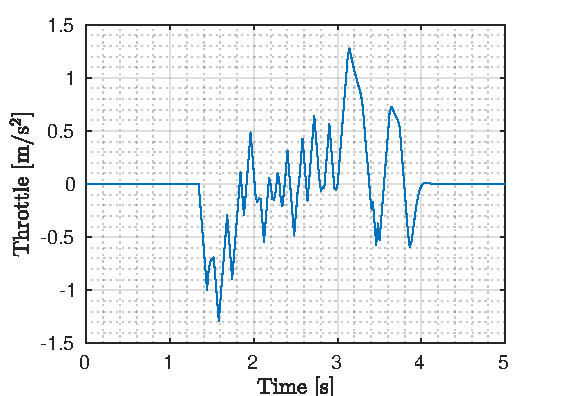
\includegraphics[width=\textwidth]{../../MATLAB/one_obstacle_right_overtaking/figure/ThrottleVsTime.pdf}
		\subcaption{}\label{fig:throttle_one_moving}
	\end{minipage}
	\begin{minipage}[t]{0.5\textwidth}
		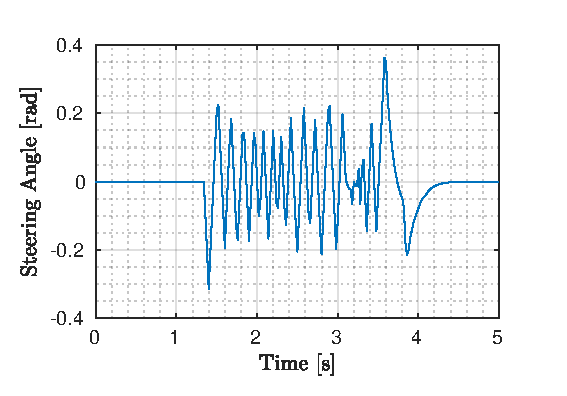
\includegraphics[width=\textwidth]{../../MATLAB/one_obstacle_right_overtaking/figure/SteeringAngleVsTime.pdf}
		\subcaption{}\label{fig:delta_one_moving}
	\end{minipage}
	\begin{minipage}[t]{0.5\textwidth}
		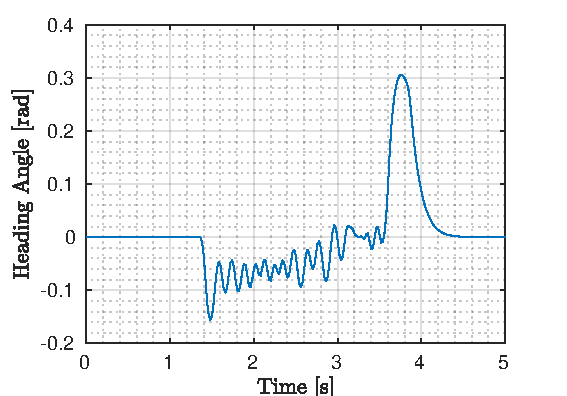
\includegraphics[width=\textwidth]{../../MATLAB/one_obstacle_right_overtaking/figure/HeadingAngleVsTime.pdf}
		\subcaption{}\label{fig:theta_one_moving}
	\end{minipage}
	\caption{Time signals of the ATLASCAR2 in the simulation of right overtaking of one moving obstacle illustrated in Figure \ref{fig:obstacleAvoidance_one_obstacle}.}
	\label{fig:components_one_moving_obstacle}
\end{figure}


%
\subsection{Multiple Moving Obstacles}
For a second test, additional obstacles were added to make the scenario more complex like in a real highway.

Initially we assumed that the obstacles were located at a distance greater than the LIDAR detection range which is \SI{30}{m}. In this way every time the vehicle overtakes a car, it applies the inactive constraints to go back to the center lane. 

This situation is represented in Figure \ref{fig:obstacleAvoidance_random}
where there are three different scenarios with $N = 2,3 \text{ and } 4$ moving obstacles that drive with a constant velocity of \SI{8}{m/s} in the opposite direction with respect to the ATLASCAR2. The vehicle is capable of overtaking the obstacles on the right or left depending on their positions with respect to the road. If the $y$-coordinate of the closest obstacle is greater than 0, then the vehicle overtakes to the right, otherwise the overtaking takes place on the left lane.
% MULTIPLE MOVING OBSTACLE
\begin{figure}[!h]
	\centering
	\begin{minipage}[t]{\textwidth}
		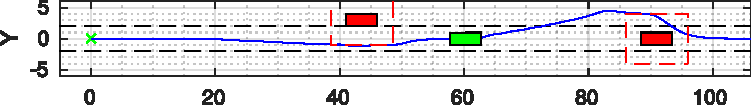
\includegraphics[width=\textwidth]{./figure/random_N_obstacles/overtaking_random_2.pdf}
	\end{minipage}
	\begin{minipage}[t]{\textwidth}
		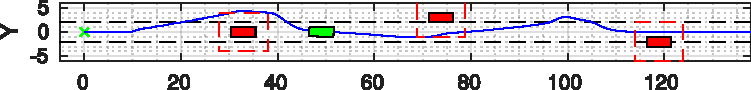
\includegraphics[width=\textwidth]{./figure/random_N_obstacles/overtaking_random.pdf}
	\end{minipage}
	\begin{minipage}[t]{\textwidth}
		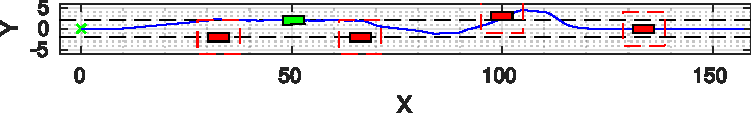
\includegraphics[width=\textwidth]{./figure/random_N_obstacles/overtaking_random_1.pdf}
	\end{minipage}
	\caption{Simulations of overtaking with $N = 2,3,4$ moving obstacles that drive in the opposite direction with respect to the ATLASCAR2.}
	\label{fig:obstacleAvoidance_random}
\end{figure}

In the Figure \ref{fig:obstacleAvoidance_six_obstacles} we also hypothesized there are six moving obstacles that can drive at different speeds but initially they are at a common distance; they can have a uniform motion or a uniformely accelerated motion. We also improved the code infact in case two obstacles are too close during the simulation and their distance is less than the detection range, which is \SI{30}{m}, the ATLASCAR2 perceives the objects as a single entity and adapts to the situation. The same test can be done with the obstacles that drive in the same direction as the vehicle but to better assess and demonstrate results we decided to show a very unusual scenario. 
% SIX MOVING OBSTACLES
\begin{figure}[b!]
	\centering
	\begin{minipage}[t]{\textwidth}
		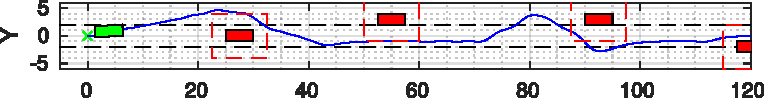
\includegraphics[width=\textwidth]{./figure/6_obstacles/6_obstacles_1.pdf}
	\end{minipage}
	\begin{minipage}[t]{\textwidth}
		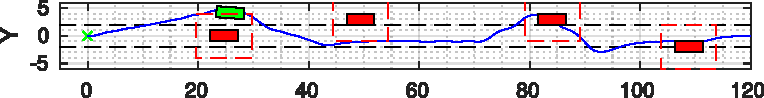
\includegraphics[width=\textwidth]{./figure/6_obstacles/6_obstacles_2.pdf}
	\end{minipage}
	\begin{minipage}[t]{\textwidth}
		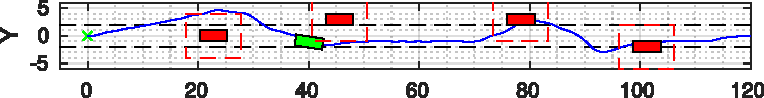
\includegraphics[width=\textwidth]{./figure/6_obstacles/6_obstacles_3.pdf}
	\end{minipage}
	\begin{minipage}[t]{\textwidth}
		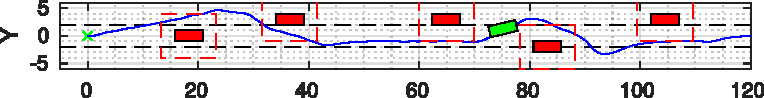
\includegraphics[width=\textwidth]{./figure/6_obstacles/6_obstacles_4.pdf}
	\end{minipage}
	\begin{minipage}[t]{\textwidth}
		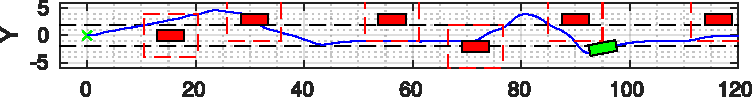
\includegraphics[width=\textwidth]{./figure/6_obstacles/6_obstacles_5.pdf}
	\end{minipage}
	\begin{minipage}[t]{\textwidth}
		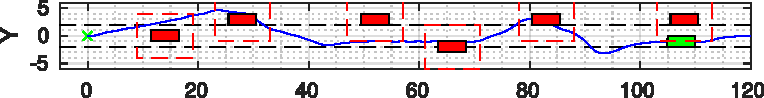
\includegraphics[width=\textwidth]{./figure/6_obstacles/6_obstacles_6.pdf}
	\end{minipage}
	\caption{Simulation of overtaking with six moving obstacles that moves in the opposite direction with respect the vehicle.}
	\label{fig:obstacleAvoidance_six_obstacles}
\end{figure}

Also in this case we reported time signals of the ATLASCAR2 in the simulation with six moving obstacles (Figure \ref{fig:components_six_moving_obstacles}). The most articulated scenario makes the signals more complex with respect to time. However, we can see that the speed is just under \SI{20}{m/s} while the inputs continue to respect the imposed boundaries. Note that the vehicle manages to overcome all the obstacles without encountering any difficulty since there is always an empty lane.
% RESULTS SIX MOVING OBSTACLES
\begin{figure}[!t] %vs changes to t instead of b
	\begin{minipage}[t]{0.5\textwidth}
		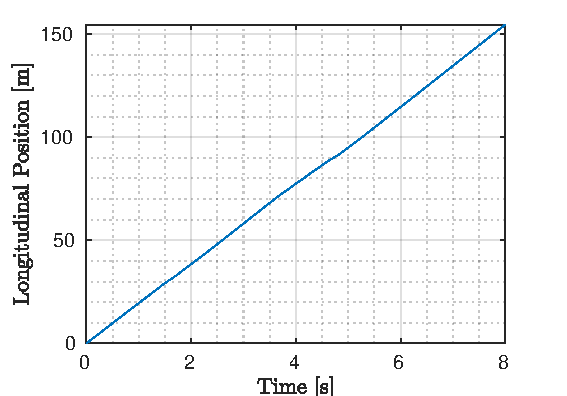
\includegraphics[width=\textwidth]{../../MATLAB/6_obstacles/figure/LongitudinalPositionVsTime.pdf}
		\subcaption{}\label{fig:longitudinal_six_moving}
	\end{minipage}
	\begin{minipage}[t]{0.5\textwidth}
		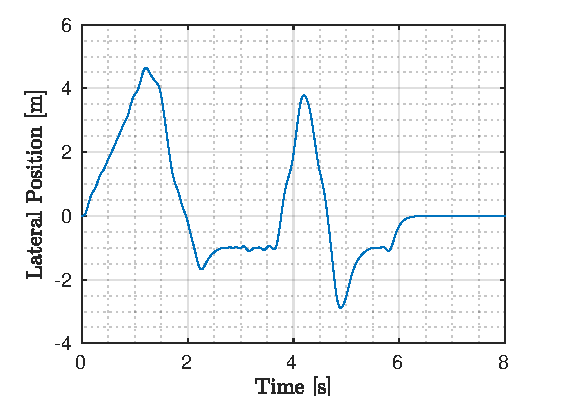
\includegraphics[width=\textwidth]{../../MATLAB/6_obstacles/figure/LateralPositionVsTime.pdf}
		\subcaption{}\label{fig:lateral_six_moving}
	\end{minipage}
	\begin{minipage}[t]{0.5\textwidth}
		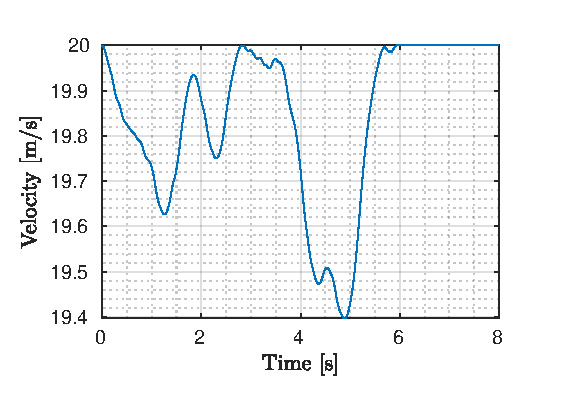
\includegraphics[width=\textwidth]{../../MATLAB/6_obstacles/figure/VelocityVsTime.pdf}
		\subcaption{}\label{fig:velocity_six_moving}
	\end{minipage}
	\begin{minipage}[t]{0.5\textwidth}
		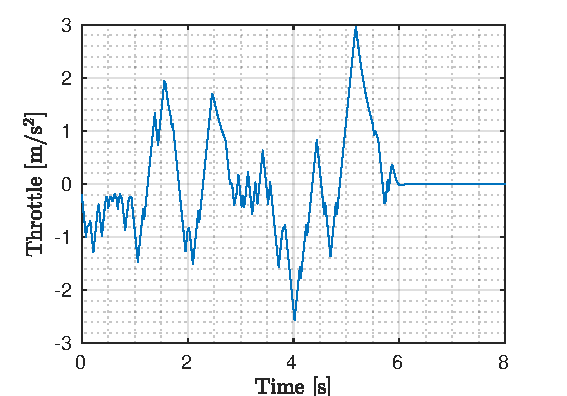
\includegraphics[width=\textwidth]{../../MATLAB/6_obstacles/figure/ThrottleVsTime.pdf}
		\subcaption{}\label{fig:throttle_six_moving}
	\end{minipage}
	\begin{minipage}[t]{0.5\textwidth}
		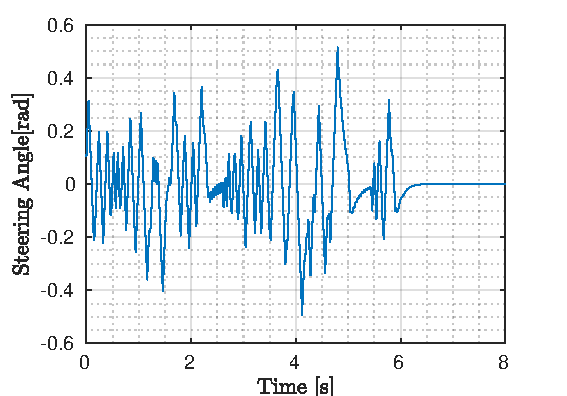
\includegraphics[width=\textwidth]{../../MATLAB/6_obstacles/figure/SteeringAngleVsTime.pdf}
		\subcaption{}\label{fig:delta_six_moving}
	\end{minipage}
	\begin{minipage}[t]{0.5\textwidth}
		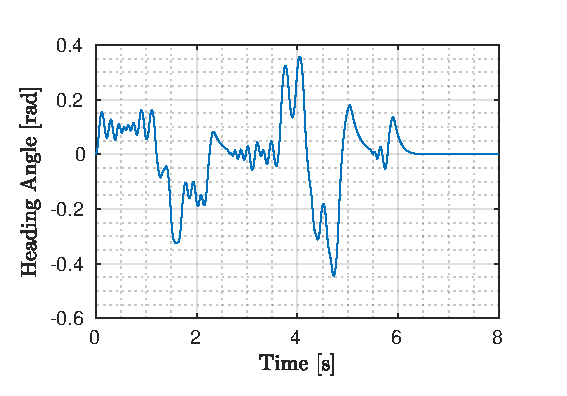
\includegraphics[width=\textwidth]{../../MATLAB/6_obstacles/figure/HeadingAngleVsTime.pdf}
		\subcaption{}\label{fig:theta_six_moving}
	\end{minipage}
	\caption{Time signals of the ATLASCAR2 in the simulation of overtaking with six moving obstacles illustrated in Figure \ref{fig:obstacleAvoidance_six_obstacles}.}
	\label{fig:components_six_moving_obstacles}
\end{figure}

\subsection{No Overtaking}
We have seen that as long as there is always a free lane, the obstacle avoidance algorithm works correctly. In the case that there are too many obstacles on the road, which do not allow overtaking, the vehicle must adapt to the situation and it must slow down in order not to collide. In the algorithm that we have developed it is possible to calculate two other restrictions which permit this deceleration in the case that it is strictly necessary. To better understand how these restrictions change the speed and deceleration of the ATLASCAR2, we simulated a scenario (Figure \ref{fig:obstacleAvoidance_no_overtaking}) in which there are 3 obstacles at an initial distance of \SI{35}{m} occupying the 3 different lanes, all with the same $x$-coordinate and the same velocity of \SI{8}{m/s}. When these obstacles enter in the vehicle's detection range, it checks whether there is enough space to perform the overtaking maneuver by calculating the distance between the obstacles. Noting that it is not possible to overtake, our vehicle must decelerate in order not to crash into the nearest car. To do this, the MPC must take into account the position of the vehicle $x_\text{min}$ and the position of the closest obstacle $x_\text{max}$.
%NO OVERTAKING
\begin{figure}[h!]
	\centering
	\begin{minipage}[t]{\textwidth}
		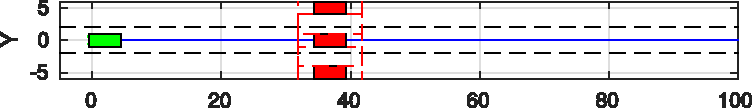
\includegraphics[width=\textwidth]{./figure/no_overtaking/no_overtaking_1.pdf}
	\end{minipage}
	\begin{minipage}[t]{\textwidth}
		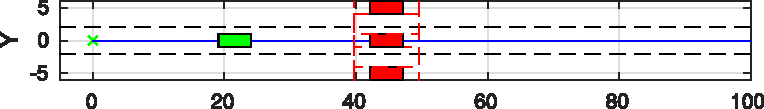
\includegraphics[width=\textwidth]{./figure/no_overtaking/no_overtaking_1_5.pdf}
	\end{minipage}
	\begin{minipage}[t]{\textwidth}
		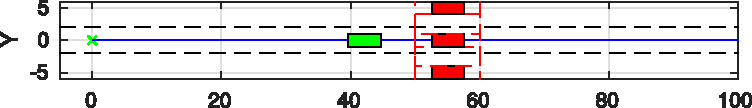
\includegraphics[width=\textwidth]{./figure/no_overtaking/no_overtaking_2.pdf}
	\end{minipage}
	\begin{minipage}[t]{\textwidth}
		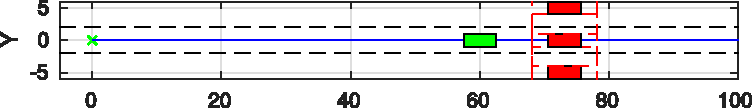
\includegraphics[width=\textwidth]{./figure/no_overtaking/no_overtaking_3.pdf}
	\end{minipage}
	\begin{minipage}[t]{\textwidth}
		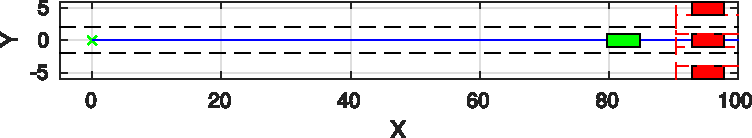
\includegraphics[width=\textwidth]{./figure/no_overtaking/no_overtaking_4.pdf}
	\end{minipage}
	\caption{Simulation of no overtaking with three moving obstacles that move in the same direction as the vehicle.}
	\label{fig:obstacleAvoidance_no_overtaking}
\end{figure}

Also in this simulation the reference speed of the car is \SI{20}{m/s}, but after $\simeq$\SI{1,5}{s}, the obstacles enter in the detection range and as we can see from the Figure \ref{fig:velocity_no_overtaking} the velocity decreases rapidly to adapt to that of the nearest vehicle. It is possible to observe that this decrease in speed, which subsequently remains constant at \SI{8}{m/s}, is due to a strong negative throttle impulse (Figure \ref{fig:throttle_no_overtaking}). Finally, we note that the steering angle $\delta$ and heading angle $\theta$ remain at zero: there is only a very small oscillatory trend due to measurement errors as the vehicle always requires a minimum change of direction.
Finally we imposed a safety distance that must always be respected between two vehicles so that if the obstacle brakes sharply the ATLASCAR2 can avoid the impact.
It is very difficult to achieve reliable calculations of the braking distance as road conditions and the tyres' grip can vary greatly. An easy formula to calculate the braking distance is the following one:
\begin{equation}
	d = \frac{v^2}{250\times f}
\end{equation}
where $d$ is the braking distance in metres, $v$ is the speed in \SI{}{km/h}, $250$ is the fixed figure which is always used and $f$ is the coefficient of friction, approx. 0.8 on dry asphalt and 0.1 on ice.
% RESULTS NO OVERTAKING
\begin{figure}[!t] %vs changes to t instead of b
	\begin{minipage}[t]{0.5\textwidth}
		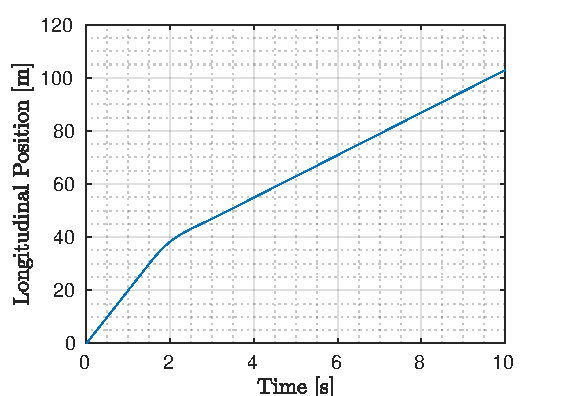
\includegraphics[width=\textwidth]{../../MATLAB/no_overtaking/figure/LongitudinalPositionVsTime.pdf}
		\subcaption{}\label{fig:longitudinal_no_overtaking}
	\end{minipage}
	\begin{minipage}[t]{0.5\textwidth}
		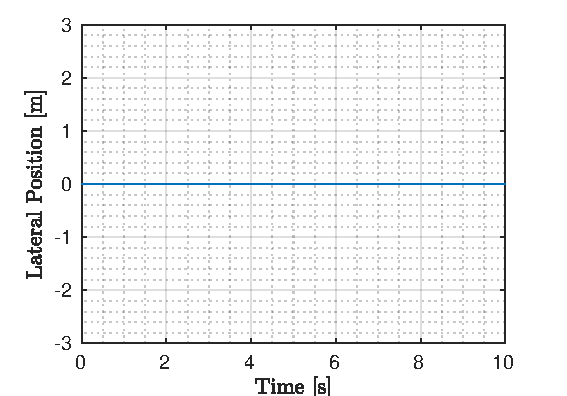
\includegraphics[width=\textwidth]{../../MATLAB/no_overtaking/figure/LateralPositionVsTime.pdf}
		\subcaption{}\label{fig:lateral_no_overtaking}
	\end{minipage}
	\begin{minipage}[t]{0.5\textwidth}
		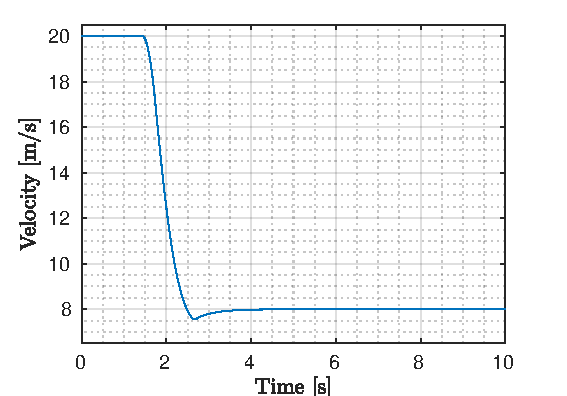
\includegraphics[width=\textwidth]{../../MATLAB/no_overtaking/figure/VelocityVsTime.pdf}
		\subcaption{}\label{fig:velocity_no_overtaking}
	\end{minipage}
	\begin{minipage}[t]{0.5\textwidth}
		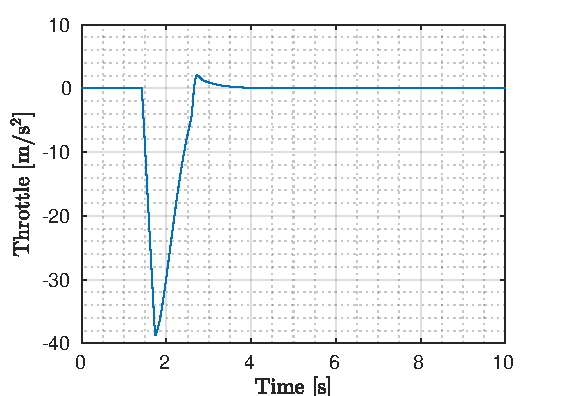
\includegraphics[width=\textwidth]{../../MATLAB/no_overtaking/figure/ThrottleVsTime.pdf}
		\subcaption{}\label{fig:throttle_no_overtaking}
	\end{minipage}
	\begin{minipage}[t]{0.5\textwidth}
		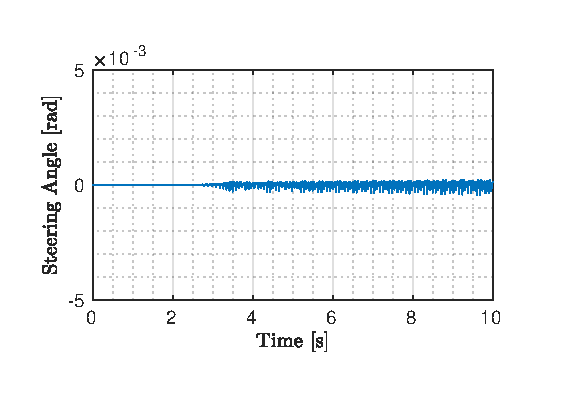
\includegraphics[width=\textwidth]{../../MATLAB/no_overtaking/figure/SteeringAngleVsTime.pdf}
		\subcaption{}\label{fig:delta_no_overtaking}
	\end{minipage}
	\begin{minipage}[t]{0.5\textwidth}
		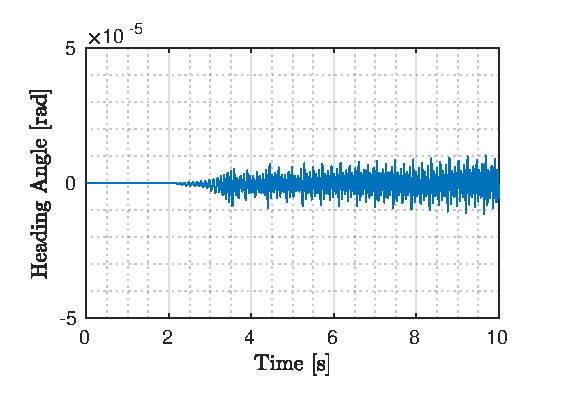
\includegraphics[width=\textwidth]{../../MATLAB/no_overtaking/figure/HeadingAngleVsTime.pdf}
		\subcaption{}\label{fig:theta_no_overtaking}
	\end{minipage}
	\caption{Time signals of the ATLASCAR2 in the simulation of no overtaking with three moving obstacles illustrated in Figure \ref{fig:obstacleAvoidance_no_overtaking}.}
	\label{fig:components_no_overtaking}
\end{figure}

\subsection{Vehicle Braking and Obstacles Overtaking}
Finally we have improved the code related to the mixed Input/Output constraints. Figure \ref{fig:braking} depicts a simulation in which there are 3 obstacles at the same $x$-coordinate. Two obstacles have a constant speed of \SI{8}{m/s} while the one on the left lane of \SI{15}{m/s}.
% BRAKING THREE OBSTACLE
\begin{figure}[!h]
	\centering
	\begin{minipage}[t]{\textwidth}
		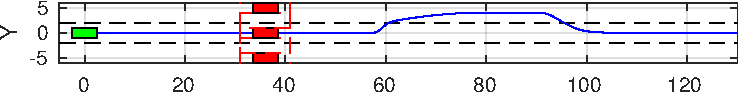
\includegraphics[width=\textwidth]{./figure/three_obstacles_no_overtaking/braking_0.pdf}
	\end{minipage}
	\begin{minipage}[t]{\textwidth}
		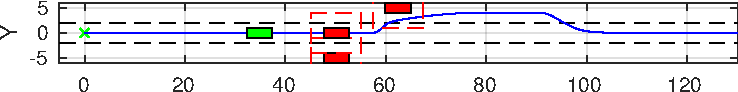
\includegraphics[width=\textwidth]{./figure/three_obstacles_no_overtaking/braking_1.pdf}
	\end{minipage}
	\begin{minipage}[t]{\textwidth}
		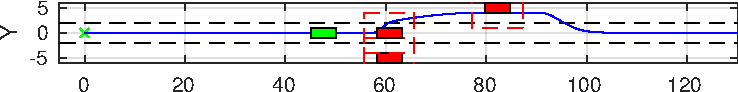
\includegraphics[width=\textwidth]{./figure/three_obstacles_no_overtaking/braking_2.pdf}
	\end{minipage}
	\begin{minipage}[t]{\textwidth}
		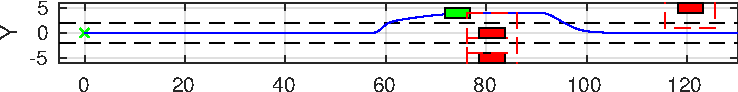
\includegraphics[width=\textwidth]{./figure/three_obstacles_no_overtaking/braking_3.pdf}
	\end{minipage}
	\begin{minipage}[t]{\textwidth}
		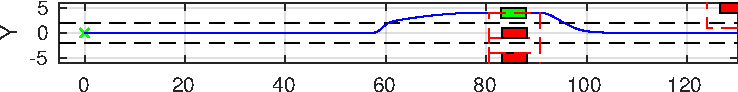
\includegraphics[width=\textwidth]{./figure/three_obstacles_no_overtaking/braking_4.pdf}
	\end{minipage}
	\begin{minipage}[t]{\textwidth}
		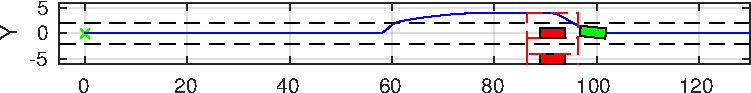
\includegraphics[width=\textwidth]{./figure/three_obstacles_no_overtaking/braking_5.pdf}
	\end{minipage}
	\begin{minipage}[t]{\textwidth}
		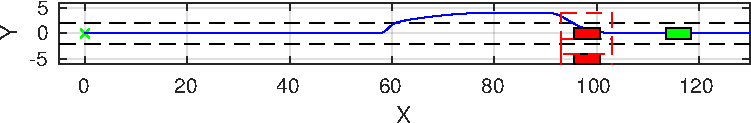
\includegraphics[width=\textwidth]{./figure/three_obstacles_no_overtaking/braking_6.pdf}
	\end{minipage}
	\caption{Simulation of braking and overtaking obstacles.}
	\label{fig:braking}
\end{figure}

In this particular case it is essential to consider the fourth and the fifth restrictions in order to allow the ATLASCAR2 to slow down without colliding with the cars in front. The fifth constraint is simply the position of the ATLASCAR2 that updates at each interval, while the fourth constraint, until there is a free lane, is the position of the closest obstacle (both the positions are with respect to the global reference frame). In the calculation of the fourth constraint is necessary  to consider the speed at which the vehicle and the obstacle are moving in order to keep a safe distance.
At the beginning, the vehicle moves with the reference velocity of $v=\SI{20}{m/s}$. When the ATLASCAR2 detects all the other cars on the road, checks if there is a free lane. In the first part of the simulation, the ATLASCAR2 brakes because there is not enough space for overtaking the cars as shown in Fig. \ref{fig:velocity_braking}. A collision would happen if the vehicle continues to follow the initially planned path with the reference velocity. It is possible to notice that the speed decreases because the applied throttle is negative, so a consistent deceleration is set after $\approx\SI{1.5}{s}$ as depicted in Fig. \ref{fig:throttle_braking}. The velocity of the ATLASCAR2 for $\approx\SI{2}{s}$ adapts to that of the closest obstacle. After a few seconds the fastest car moves and makes available the left lane for overtaking. Dramatic changes of steering angle in early stage are observed in Fig. \ref{fig:delta_braking} and consequently also on the heading angle in Fig. \ref{fig:theta_braking}. Then, the ATLASCAR2 returns to the reference velocity during the overtaking of the two obstacles (the applied throttle after $\approx\SI{5}{s}$ is positive). It is seen that the ATLASCAR2 avoids the obstacles and returns to the road center line with a low overshoot.

% RESULTS BRAKING THREE OBSTACLES
\begin{figure}[!h] %vs changes to t instead of b
	\begin{minipage}[t]{0.5\textwidth}
		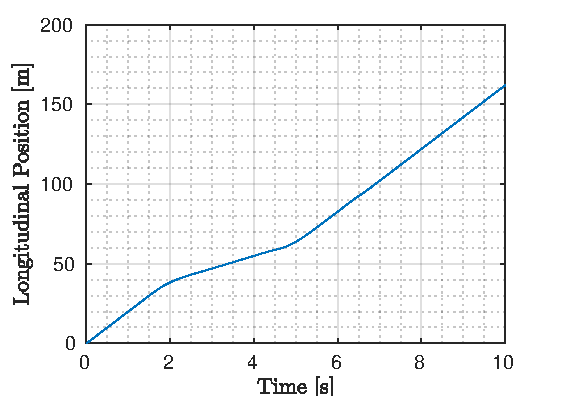
\includegraphics[width=\textwidth]{./figure/three_obstacles_no_overtaking/LongitudinalPositionVsTime.pdf}
		\subcaption{}\label{fig:longitudinal_braking}
	\end{minipage}
	\begin{minipage}[t]{0.5\textwidth}
		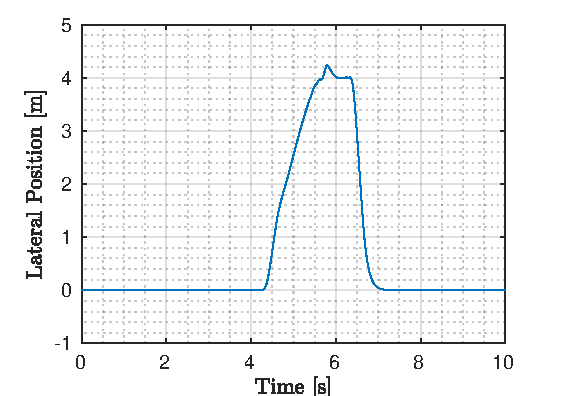
\includegraphics[width=\textwidth]{./figure/three_obstacles_no_overtaking/LateralPositionVsTime.pdf}
		\subcaption{}\label{fig:lateral_braking}
	\end{minipage}
	\begin{minipage}[t]{0.5\textwidth}
		\includegraphics[width=\textwidth]{./figure/three_obstacles_no_overtaking/VelocityVsTime.pdf}
		\subcaption{}\label{fig:velocity_braking}
	\end{minipage}
	\begin{minipage}[t]{0.5\textwidth}
		\includegraphics[width=\textwidth]{./figure/three_obstacles_no_overtaking/ThrottleVsTime.pdf}
		\subcaption{}\label{fig:throttle_braking}
	\end{minipage}
	\begin{minipage}[t]{0.5\textwidth}
		\includegraphics[width=\textwidth]{./figure/three_obstacles_no_overtaking/SteeringAngleVsTime.pdf}
		\subcaption{}\label{fig:delta_braking}
	\end{minipage}
	\begin{minipage}[t]{0.5\textwidth}
		\includegraphics[width=\textwidth]{./figure/three_obstacles_no_overtaking/HeadingAngleVsTime.pdf}
		\subcaption{}\label{fig:theta_braking}
	\end{minipage}
	\caption{Time signals of the ATLASCAR2 in the simulation of braking and overtaking in the situation illustrated in Figure \ref{fig:braking}.}
	\label{fig:components}
\end{figure}
